\section{Introduction}
\label{sec:Introduction}

Construction industry is becoming increasingly data intensive with the growing use of
information and communication technology in all phases of a building life-cycle. 
In the future, buildings will act as hubs of a wide variety of real-time and accumulated data about
spaces, indoor locations, indoor routes, assets, people, sensors, materials, equipment, connections
to surrounding networks (traffic, infrastructure, communication), detected issues, and 
activities in the building.

Currently, huge amounts of information about building designs is produced  
using Building Information Modeling (BIM) tools \cite{eastman2011bim}. A widely adopted standard, 
IFC (Industry Foundation Classes) \cite{ISO16739,liebich2010unveiling} provides a common representation for BIM models of 
different design disciplines. All major BIM tools support IFC and can export BIM models to IFC files for exchange with other parties.

BIM models could provide a natural framework to organize and manage building related information. However, a big obstacle is the difficulty to access and utilize BIM models which have traditionally been shared through point-to-point file exchange. They cannot be used in an online, granular, and 
interlinked manner. This provides a poor basis for open utilization of building information and the 
emergence of new, innovative applications.
To make BIM models accessible on the Web \cite{torma2014wobd}, we have developed the 
\bname{WebIFC converter} to 
derive OWL ontologies from the IFC schema (\ifcowl{}), and RDF datasets from IFC files 
(\ifcrdf{}). The \ifcowl{} specifies concepts, relations, and constraints for \ifcrdf{} datasets that replicate the content of IFC files. 
All terms defined in \ifcowl{}  must thus be based on the corresponding constructs in 
the IFC schema. 

\begin{figure}[h]
\centering
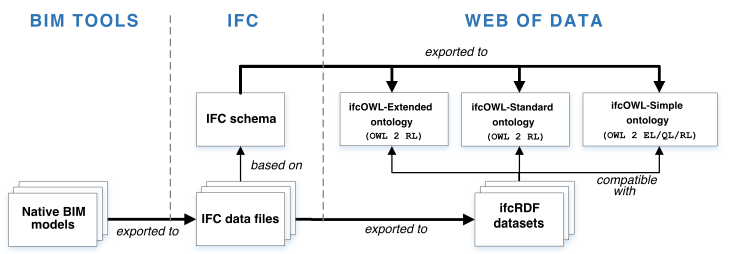
\includegraphics[angle=0,width=1.0\textwidth]{images/ifcOWL-multilayers.png}
%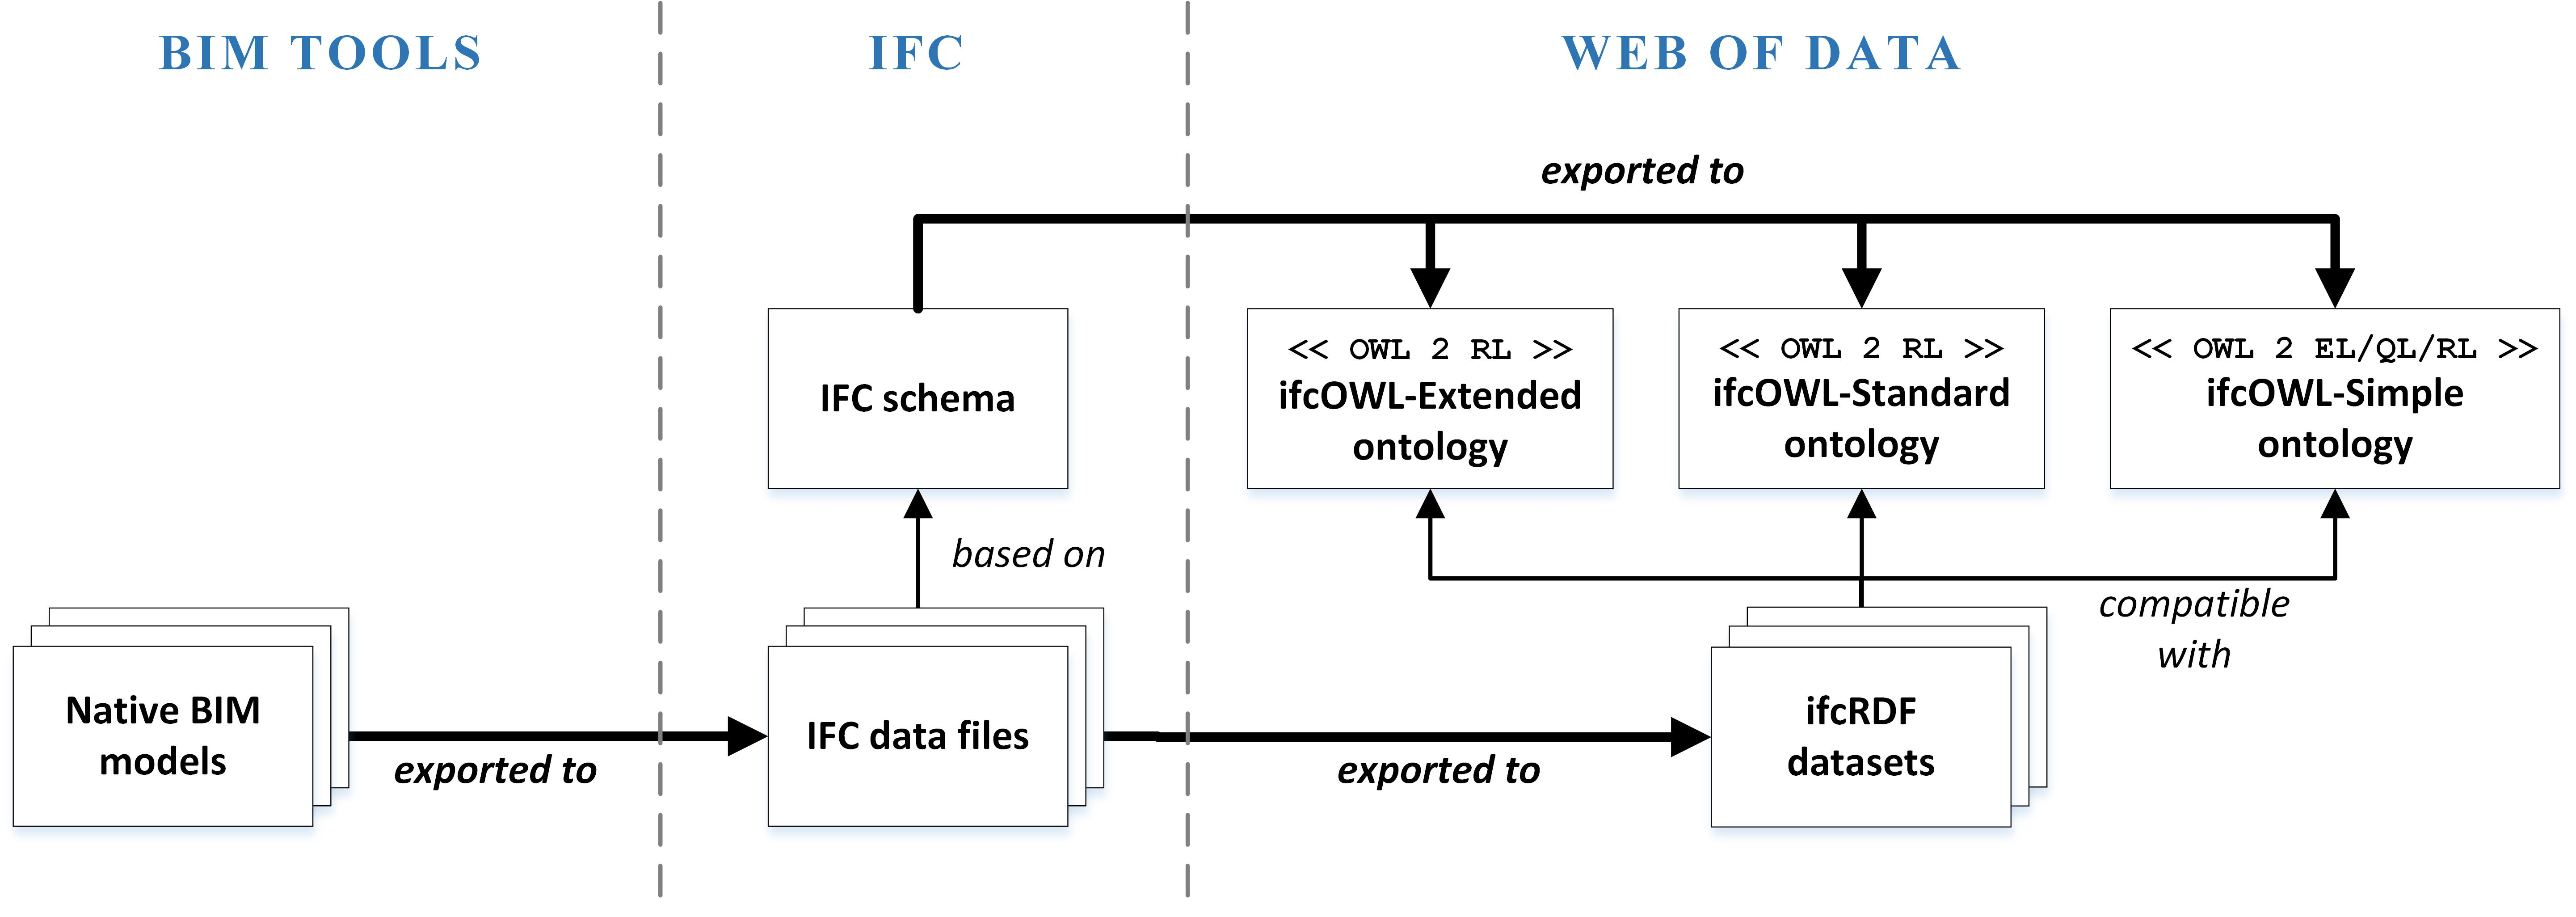
\includegraphics{images/ifcOWL-multilayers.jpg}
\caption{Multiple layers of \ifcowl{} ontology}
\label{fig:ifcOWL-layers}
\end{figure}

The conversion of IFC files to \ifcrdf{} is straightforward and can be done 
without information loss.
Ideally, there would also be just one \ifcowl{} ontology for each version of the IFC schema. However,
there are possibilities and reasons to convert the IFC schema to OWL in several different ways. Firstly, there is a \emph{mismatch} between the modeling constructs of OWL and 
EXPRESS data definition language \cite{schenck1994information} used to specify the IFC schema. Secondly, a simple version of \ifcowl{} \emph{compatible with
restricted OWL profiles} (OWL 2 EL or QL) \cite{motik2012owl} is useful to support ontology
reasoning or inexact reasoning. Thirdly, for most practical purposes only a subset of ontology
information is required, as no validation or checking of \ifcrdf{} data is needed; it can
be considered \emph{practically valid} w.r.t. the schema, since BIM tools use certified converters. Moreover, icfRDF can sensibly only be used in a
\emph{read-only} fashion, since BIM models will be maintained in the native formats of BIM
tools. In addition, a full conversion of the IFC schema produces a huge ontology, difficult to understand or manipulate.

Consequently, we convert the IFC schema into a \emph{flexible, multilayer \ifcowl{} ontology}
in a way that \emph{\ifcrdf{} is compatible with any of the layers} (Fig. \ref{fig:ifcOWL-layers}). 
New representational constructs are introduced at more comprehensive levels which therefore 
provide increasing detailed type information about \ifcrdf{} data: 

\vspace{0.5\topsep}
\noindent
\begin{scriptsize}
\begin{center}
    \def\arraystretch{1.2}
    \setlength{\tabcolsep}{6pt}
    \begin{tabularx}{0.95\textwidth}{|l|l|X|}
        \hline
            \textbf{Layer} & \textbf{Profile} & \textbf{Included schema information} \\
        \hline
            ifcOWL-Simple & OWL 2 EL or & Schema meta data plus: \\
            & OWL 2 QL or & \ \ - All type definitions and hierarchies \\
            & OWL 2 RL & \ \ - All entity type properties (names, range types) \\
        \hline 
            ifcOWL-Standard & OWL 2 RL & All above plus: \\
            & & \ \ - All entity type keys \\
            & & \ \ - All entity type inverse properties \\
        \hline
            ifcOWL-Extended & OWL 2 RL & All above plus: \\
            & & \ \ - All cardinality constraints \\
        \hline
    \end{tabularx}
\end{center}
\end{scriptsize}

%Since all \ifcrdf{} datasets are compatible with all layers of the \ifcowl{} ontology 
%(Fig. \ref{fig:ifcOWL-layers}), the most appropriate one can be selected based on the requirements of 
%a use case and tools. For instance, many Linked Data applications that need to 
%query entity properties, use the type hierarchy, or convert \ifcrdf{} datasets back to 
%object-oriented data models it is sufficient to use the \name{ifcOWL-Simple} ontology. 
%In case of reasoning about data that includes inverse properties, it is recommended to use 
%\name{ifcOWL-Standard} ontology. If an RDF dataset needs to be modified and data validated 
%using type and cardinality constraints, \name{ifcOWL-Extended} is the correct choice.


From the previous IFC-to-OWL/RDF conversions
\cite{beetz2005ontology,beetz2009ifcowl,pauwels2011interoperability} our approach differs since it
is based on OWL 2 profiles, produces a flexible multilayer ontology, applies \emph{very different methods of data\-type definitions} and is specifically targeted to
real-life Linked Data applications. It uses stable URIs for entities, in contrast to the previous approaches
where the URIs were instable across models versions.

CityGML \cite{kolbe2005citygml} is a surface model for buildings, which can be useful to visitors for 
indoor navigation. IFC contains complementary information about building design, structure, 
and equipment for a wider range of stakeholders and use cases. Moreover, IFC data can be one source 
when generating CityGML models. % GityGML has also been converted into OWL. 

In the rest of this paper we describe the conversions to \ifcowl{} and \ifcrdf{}, present the deployment of ontologies, example datasets and the converter, and finish with summary and future work. 


% \begin{figure}
% \centering
% %\def\svgwidth{\textwidth}
% \def\svgscale{1}
% \input{images/image.pdf_tex}
% %{\includesvg{images/test-2}}
% %\includegraphics[width=0.75\textwidth]{images/ifcOWL-multilayer-2.png}
% \caption{A multilayer ifcOWL ontology}
% \label{fig:ifcOWL-multilayered}
% \end{figure}